\section{Transporting complete boxes}
\label{sec:bb-boxes}

We allow an instruction to change all three side lengths while
preserving their product. The geometric question is concrete:
given finitely many disjoint closed boxes and prescribed determinant-one
affine maps onto another disjoint family, can one carry out every map by
a smooth incompressible motion?  The two families may overlap each
other.  Consequently a destination cannot be occupied until every source
that obstructs it has been removed.

We first extend an explicitly separated motion to a velocity field.
We then give two ways to produce that motion.  Separate horizontal
projections permit a simple lift and transfer.  For general solid boxes
we use parking and detours around the other occupied boxes.
Figure~\ref{fig:bb-routing} contrasts the height separation with the
evacuation order that makes overlapping source and target families harmless.

\subsection{An affine motion and its curl extension}

Throughout, a smooth switch is obtained by translating and rescaling
$\sigma$ in \eqref{eq:p2-step}, with its transition strictly inside
its allotted interval.  Thus successive motions are stationary on
neighborhoods of their joining times.

\begin{lemma}[A velocity on a neighborhood of each moving box]
\label{lem:bb-curl}
Let $K_i(t)=c_i(t)+D_i(t)K_i^0$, $1\le i\le N$, where $K_i^0$ is
an axis-parallel box, possibly with zero side lengths, and $D_i(t)$ is
positive diagonal with determinant one.  Suppose the centers and scales
are smooth and constant near the ends of a compact time interval.
For the effective conclusion, assume computable endpoints for the
initial boxes $K_i^0$, effective evaluation of the centers' and scales'
derivatives, bounds for those derivatives, and positive lower bounds
for every scale on that interval.
If the coordinatewise $2\eta$ enlargements of the moving boxes are
pairwise disjoint and bounded, for a known $\eta>0$, a
compactly supported smooth divergence-free field realizes these motions
on open neighborhoods of the initial boxes.  It vanishes near the time
endpoints.  When all enlarged boxes lie in an interior torus chart,
the field extends to a mean-zero field on that torus.
The field is effective under the effective-data assumptions above;
smooth existence itself does not require computable data.
\end{lemma}
\begin{proof}
Choose a smooth cutoff $\chi_i$ which is one on the $\eta$
enlargement of $K_i(t)$ and supported in its $2\eta$ enlargement,
using products of the effective switches.  Put $y=x-c_i$ and
$L_i=\dot D_iD_i^{-1}$; then $\operatorname{tr}L_i=0$.
Take the curl of
\begin{equation}\label{eq:bb-potential}
 \chi_i\{\tfrac12\dot c_i\times y+\tfrac13(L_i y)\times y\}.
\end{equation}
The identity
$\nabla\times(G\times y)=2G-y\operatorname{div}G+(y\cdot\nabla)G$
shows that this curl equals $\dot c_i+L_i y$ on the plateau.
Disjoint supports permit summation over $i$.  The path
$c_i(t)+D_i(t)D_i(t_0)^{-1}(x_0-c_i(t_0))$ has exactly that
derivative and remains in its prescribed box.  ODE uniqueness proves
the formula.  On the compact time interval the normalized matrix norm
has a finite bound $M$, computable under the effective-data assumptions;
an initial perturbation less than
$\eta/(2M)$ remains on the plateau.  This proves the neighborhood
claim, also for zero-width initial boxes.
The potential is zero near time endpoints because the centers and
scales are constant there.  Its support is bounded.  Within a torus
chart extend the potentials by zero; periodic curls have zero integral.
\end{proof}

\begin{proposition}[Fluid realization and a pressure refinement]
\label{prop:bb-realization}
Fix $\nu>0$.  A finite collection of the preceding motions, repeated
with period one, or preceded by one finite loading interval, yields a
smooth prescribed velocity $U$ with $U(0)=0$.  Suppose its spatial
support is contained in one compact set in $\R^3$, or its potentials
are contained in interior torus charts.  Then
\begin{equation}\label{eq:bb-residual}
 f=U_t+(U\cdot\nabla)U-\nu\Delta U
\end{equation}
has the same support and time periodicity and bounded mixed derivatives
of every order.  The solution is $(U,0)$, with the uniqueness and
material-flow conclusions of Lemma~\ref{lem:p2-realization}.
In $\R^3$ its uniqueness statement also holds when the competing
pressure has an $H^1$ representative at each time, without requiring
continuity into $H^1$, while the other velocity hypotheses of
Section~\ref{sec:model} are retained.  On the torus $U$ and $f$ have
zero mean. Under the effective-data assumptions of Lemma~\ref{lem:bb-curl},
the formula is $f_0+\nu f_1$ with effective coefficients;
evaluation is effective for computable $\nu$, and relative to $\nu$
otherwise.
\end{proposition}
\begin{proof}
The residual identity and Lemma~\ref{lem:b-comparison} give existence,
uniqueness and the material flow.  In the whole-space pressure refinement
use case (ii): the reference field has compact support and smooth bounded
mixed derivatives, hence belongs to $CH^2\cap C^1L^2$ with bounded
velocity and gradient; the competing velocity and pointwise $H^1$
pressure are exactly that case's hypotheses.  No pressure continuity
in time is added.  Integrating the residual on a torus uses
$\int U=0$, $\int\Delta U=0$ and
$\int(U\cdot\nabla)U=\int\operatorname{div}(U\otimes U)=0$.

Each derivative of $e^{-1/s}$ for $s>0$ is a polynomial in $1/s$
times $e^{-1/s}$.  The estimate
$v^m e^{-v}\le(m+k)!v^{-k}$ supplies effective endpoint error bounds,
and the denominator defining $\sigma$ is at least $e^{-2}$.
Under those effective-data assumptions all positive scales have effective
positive lower bounds. Finite
compositions, differentiation, and the logarithms of positive computable
scales are therefore effective.  At an approximate time, a coarse bound
gives a finite superset of possible translates of the zero-extended
unit template.  This evaluates the periodic field without deciding
whether time is an integer.  None of these operations iterates the
machine execution: the program contains the entire finite instruction
list.
\end{proof}

\subsection{Three geometric schedules}

For later use we describe the exact hypotheses of the schedules.
First suppose $P_i,Q_i\subset\R^2$ are finite families of closed
rectangles, possibly with zero side lengths, separately
pairwise disjoint, with affine maps
\[
 F_i(x)=q_i+\operatorname{diag}(\lambda_i,\lambda_i^{-1})(x-p_i),
 \qquad \lambda_i>0,
\]
where $p_i,q_i$ are their centers, and require $F_i(P_i)=Q_i$.
Their side lengths have a common finite bound. Source and target rectangles
belonging to different families need not be disjoint. The smooth existence
statements allow arbitrary real rectangle coordinates and scales. For the
effective conclusions, assume rational rectangle endpoints and rational
scales, together with computable chosen heights and vertical half-widths;
then a rational side-length bound and positive gap margins can be computed.

\begin{lemma}[Separated projections and parking]
\label{lem:bb-lift-parking}
These reciprocal maps have the following smooth compactly supported
unit-time realizations, stationary on time collars. They are effective
under the rational-data assumptions just stated.
\begin{enumerate}
\item For the products $P_i\times[z_0-h,z_0+h]$, with common $h\ge0$
and $z_0\in\R$, lift all boxes with their source projections fixed,
transfer them at sufficiently separated private heights, and lower
them with their target projections fixed.  The middle motion may use
$g_i(s)=\lambda_i^s$ or $g_i(s)=1+s(\lambda_i-1)$ and matrix
$\operatorname{diag}(g_i,g_i^{-1},1)$, with the center interpolated
linearly in $s$.  Each horizontal width stays between its endpoint
widths.  In the linear case every point satisfies
\begin{equation}\label{eq:bb-convex-coordinate}
 X_1(s)=(1-s)X_1(0)+sX_1(1).
\end{equation}
\item Alternatively, choose disjoint parking rectangles away from both
families.  Move every source to its parking site before delivering any
target, using an upward, horizontal, and downward translation.  Reshape
at the parking sites, then deliver by the same three translations.
This uses $7N$ motions. The same schedule applies to assigned onto positive
diagonal determinant-one maps between rational solid boxes whose centers
lie in a common horizontal plane and whose source and target horizontal
projections are separately disjoint. Require both horizontal widths during
reshaping to stay inside their reserved parking rectangles and the travel
height above the common plane to exceed twice the largest vertical
half-width.
\end{enumerate}
Both constructions act on neighborhoods of the whole source boxes.
\end{lemma}
\begin{proof}
In the first construction choose padding smaller than a quarter of
the within-family horizontal gaps and choose height differences larger
than twice the padded vertical half-width.  During lift and descent,
horizontal separation suffices.  During transfer, vertical separation
suffices.  The two choices of $g_i$ are positive and monotone between
$1$ and $\lambda_i$; their reciprocals are monotone as well.  Thus the
width claim holds.  The affine path is
$c_i(s)+\operatorname{diag}(g_i,g_i^{-1},1)(X_0-c_i(0))$.
Its first coordinate gives \eqref{eq:bb-convex-coordinate} exactly for
the linear choice.  Lemma~\ref{lem:bb-curl} now applies.

For the second construction choose padding smaller than the gaps in
each union of source projections with reserved parking rectangles, and
of target projections with those rectangles.  In the evacuation pass,
vertical motion is separated from uncollected sources and parked boxes.
During delivery it is separated from already filled targets and boxes
still parked.  At travel height, the moving box is above every resting
box.  A shape change stays within its own reserved projection.
These are the occupied sets at each actual time; source--target
intersection causes no interference because all sources have left
before delivery starts.  Lemma~\ref{lem:bb-curl} applies to each motion
with every other box fixed.  Finite concatenation gives the required
neighborhood map.
\end{proof}

\begin{figure}[ht]
\centering
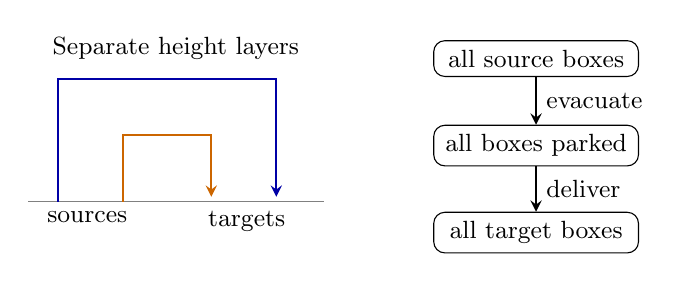
\begin{tikzpicture}[x=.75cm,y=.65cm,>=stealth,font=\small]
 \draw[gray] (0,0)--(5,0);
 \draw[thick,blue!65!black,->] (.5,0)--(.5,2.4)--(4.2,2.4)--(4.2,.1);
 \draw[thick,orange!80!black,->] (1.6,0)--(1.6,1.3)--(3.1,1.3)--(3.1,.1);
 \node[below] at (1,0) {sources};
 \node[below] at (3.7,0) {targets};
 \node[above] at (2.5,2.6) {Separate height layers};
 \begin{scope}[xshift=5.1cm]
  \node[draw,rounded corners,minimum width=2.6cm] (s) at (1.8,2.8) {all source boxes};
  \node[draw,rounded corners,minimum width=2.6cm] (p) at (1.8,1.1) {all boxes parked};
  \node[draw,rounded corners,minimum width=2.6cm] (t) at (1.8,-.6) {all target boxes};
  \draw[->,thick] (s)--(p) node[midway,right] {evacuate};
  \draw[->,thick] (p)--(t) node[midway,right] {deliver};
 \end{scope}
\end{tikzpicture}
\caption{The two separation mechanisms in
Lemma~\ref{lem:bb-lift-parking}.  Left: horizontal projections separate
the lift and descent, and distinct heights separate the transfer;
the second horizontal coordinate is suppressed.  Right: a temporal
schedule, not a spatial drawing.  Every source is removed before any
target is occupied, so overlap between the two families is harmless.}
\label{fig:bb-routing}
\end{figure}

There is also a useful stream-function implementation of the first
schedule.  Suppose $a_i,a_i'$ are the lower left corners of $P_i,Q_i$.
At height $z_i$, put $d_i=a_i'-a_i$, $b_i=\log\lambda_i$ and
$g_i(s)=a_i+sd_i$.  On a neighborhood of the swept rectangle use
\begin{equation}\label{eq:bb-mid-stream-path}
 \xi_i(s)=g_i(s)+\operatorname{diag}(\lambda_i^s,\lambda_i^{-s})(\xi-a_i).
\end{equation}
The Hamiltonian
\[
 H_i=d_{i1}y-d_{i2}x+b_i(x-g_{i1})(y-g_{i2})
\]
generates this motion. Put $\widehat H_i=\chi_iH_i$, where $\chi_i$
is one near the whole sweep and supported in its reserved layer. Use
\[
 \dot s(\partial_y\widehat H_i,-\partial_x\widehat H_i,0).
\]
Disjoint height layers separate these cutoffs.  Vertical phases use
$\nabla\times(0,x\chi_i,0)$, equal to $(0,0,1)$ on their column
plateaus.  If $M=\max_i(1,\lambda_i,\lambda_i^{-1})$ and the column
plateau margins are $\delta,\delta'$, an initial thickening smaller than
$\min(\delta/(4M),\delta'/(4M),1/(8M))$ stays on every plateau.
Thus the affine formula also holds on open neighborhoods. For points of
the original rectangle it has the additional bound
\begin{equation}\label{eq:bb-mid-stream-safe}
 X_1(s)\ge\min(a_{i1},a'_{i1}).
\end{equation}
The bound follows because the first relative coordinate in
\eqref{eq:bb-mid-stream-path} is nonnegative.

\subsection{Solid boxes with overlapping projections}

The preceding lift requires separate horizontal projections.  We now
remove that restriction; this is needed when all three coordinates
encode independent stacks.

\begin{theorem}[Expansion, obstacle detours, and delivery]
\label{lem:bb-balanced-box-routing}
Let $Q_i=a_i+\prod_{j=1}^3[-h_{ij},h_{ij}]$ and
$Q_i'=b_i+\prod_{j=1}^3[-k_{ij},k_{ij}]$ be rational solid boxes,
with positive half-widths, each family pairwise disjoint.  Suppose
$s_{ij}=k_{ij}/h_{ij}$ and $\prod_js_{ij}=1$.  An effective compactly
supported smooth solenoidal field, zero outside the time interval
$[1/4,3/4]$, has time-one map
\[
 a_i+y\longmapsto b_i+\operatorname{diag}(s_{i1},s_{i2},s_{i3})y
\]
on a neighborhood of each $Q_i$.
\end{theorem}
\begin{proof}\label{proof:bb-balanced-box-routing}
For an empty family take the zero field.  Otherwise let
$R=\max(1,h_{ij},k_{ij})$.  Choose a rational $\Lambda>10$ so that
centers in each of the lists $(\Lambda a_i)$ and $(\Lambda b_i)$
are separated by more than $20R$ in maximum norm.  This is possible
because distinct disjoint boxes have distinct centers.  Let
\[
 K=\max(4\Lambda,|\Lambda a_{i1}|,|\Lambda b_{i1}|),
 \qquad d_i=(K+30Ri,0,0).
\]
The $d_i$ are parking centers, separated from each other and both scaled
families by at least $30R$ in their first coordinate.

First multiply all source centers by a common factor increasing from
$1$ to $\Lambda$, while keeping shapes fixed.  Next change all shapes
at those separated centers by factors $s_{ij}^{\theta}$,
$0\le\theta\le1$.  Each half-width is the geometric interpolation
$h_{ij}^{1-\theta}k_{ij}^{\theta}\le R$.
Move the boxes one at a time from $\Lambda a_i$ to $d_i$, then,
after all have been parked, from $d_i$ to $\Lambda b_i$.
Finally shrink all target centers by a common factor from $\Lambda$
to $1$, with target shapes fixed.

Here is a finite construction of every single-box path.  Around each
stationary center place the closed cube of maximum-norm radius $4R$.
These cubes are disjoint since stationary centers are separated by
more than $20R$, and neither endpoint is in a cube.  Start with the
straight segment between the endpoints.  Its intersections with the
cubes are rational intervals, found by linear inequalities.  Replace
each portion inside a cube by a polygonal path on its boundary: join
the entry point to a vertex of a containing face, use cube edges to a
face containing the exit point, and join to that exit point.  The cube
is convex face by face, so these segments remain on its boundary;
no other cube meets them.  A tangency needs no replacement.  The
resulting rational polygonal path has distance at least $4R$ from
every stationary center.  Traverse its segments with flat switches,
stopping to all orders at vertices.  Its geometric image is unchanged,
so smoothing the time parameter does not reduce clearance.

For a uniform localization margin, let $g_a$ be the minimum over
$i<j$ of
\[
 \max_\ell(|a_{i\ell}-a_{j\ell}|-h_{i\ell}-h_{j\ell}),
\]
and define $g_b$ similarly.  These are positive; for a singleton list
set both to $R$.  During outward expansion a separating coordinate
gap can only increase; during final contraction the target gap is its
minimum.  During deformation centers are more than $20R$ apart.
During a single-box path the center distance is at least $4R$, leaving
a coordinate gap at least $2R$.  Hence padding smaller than
$\tfrac18\min(R,g_a,g_b)$ satisfies Lemma~\ref{lem:bb-curl}
throughout.  Put all stages, and all straight segments, in consecutive
subintervals of $[1/4,3/4]$.  Their flat switches give a smooth finite
motion, with positive diagonal determinant-one linear parts.  That
lemma provides the velocity and the neighborhood assertion.  All
choices use rational inequalities and effective elementary functions,
which also supply bounds for every derivative.
\end{proof}
